\section{Coupled System}

\subsection{Testing}
Before we investigate the effects of increasing the coupling strength between the two systems, we verify that if the hopping amplitude $v_c = 0$, the spectra on the individual sites remain unchanged. For the coupled system, calculating the Lehmann spectrum is no longer an option as memory becomes a limiting factor; instead, we resort to using the Green's function method.

\medskip
This is indeed the case, as can be seen when comparing Fig. \ref{fig:coupled_vc_0} with the spectra in Fig. \ref{fig:spectrum_engineering} and Fig. \ref{fig:isolated_benzene}. The slight variations being due to a difference in parameters used to perform the Fourier transformation.

\begin{figure}[!hbt]
    \centering
    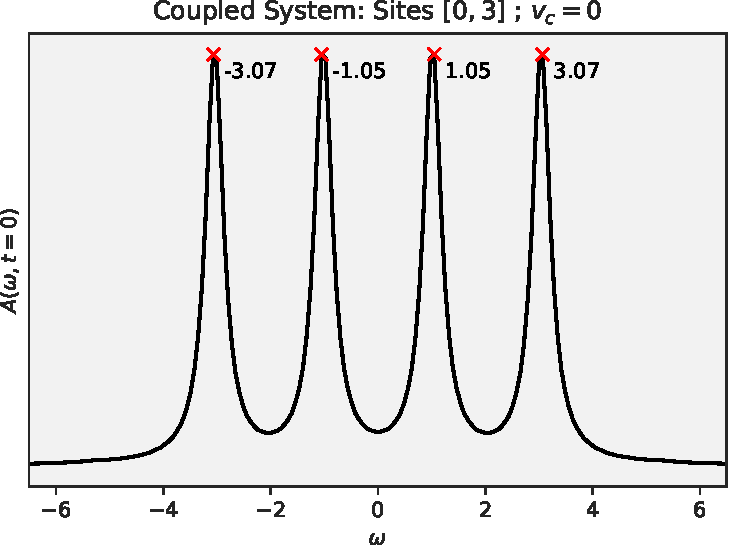
\includegraphics[width=0.47\textwidth]{graph/coupled_QD_vc_0.pdf}
    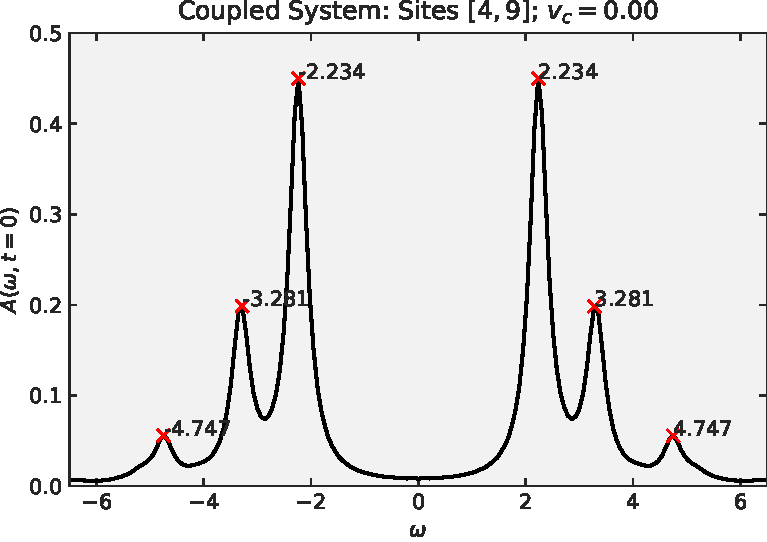
\includegraphics[width=0.47\textwidth]{graph/coupled_benzene_vc_0.pdf}
    \caption{Spectral function of all the sites of the coupled system with the coupling parameter turned off, $v_c = 0$. These spectra should be identical to those in Fig. \ref{fig:spectrum_engineering} and Fig. \ref{fig:isolated_benzene}}
    \label{fig:coupled_vc_0}
\end{figure}

\subsection{Dependence of the spectrum on the coupling strength}
Fig. \ref{fig:spectrum_vc_sweep_QD} and Fig. \ref{fig:spectrum_vc_sweep_benzene} show how the spectrum changes on each site as the coupling strength $v_c$ between the QD and the benzene ring increases. Notice that the symmetry of the geometry is preserved, as all QD sites show the same spectra. The benzene site pairs 5, 9 and 6, 8 also each share identical spectra since they are symmetric about site 4, which is the one coupled to the QD.
\medskip

In the spectrum of site $4$ in Fig. \ref{fig:spectrum_vc_sweep_benzene}, it is particularly evident that for larger $v_c$, the lower bands (below $\omega=0$) become hybridised, meaning that the energy levels from the isolated systems shift towards each other, creating a new state. The reason this only happens for the lower bands has to do with the symmetry of the systems being broken upon allowing hoppings between the QD and benzene.
\medskip

Another interesting effect that can be seen in Figs. \ref{fig:spectrum_vc_sweep_QD} and \ref{fig:spectrum_vc_sweep_benzene} is that as $v_c$ increases, the spectra experience a slight shift in energy. For the QD, the shift is towards lower energies, and for benzene, it is in the opposite direction. A possible explanation for this is given in \ref{subsec:electron_transfer_QD_benzene}.

\begin{figure}[!hbt]
    \centering
    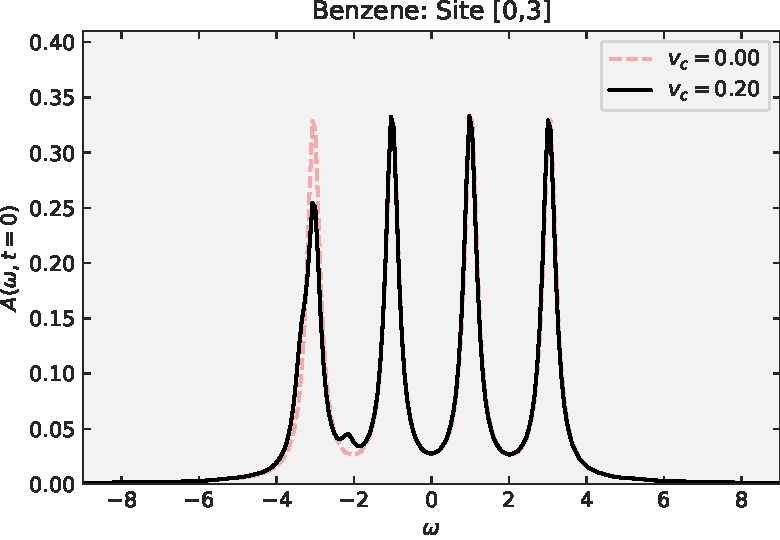
\includegraphics[width=0.49\textwidth]{graph/spectrum_vc_sweep/QD_All_020.pdf}
    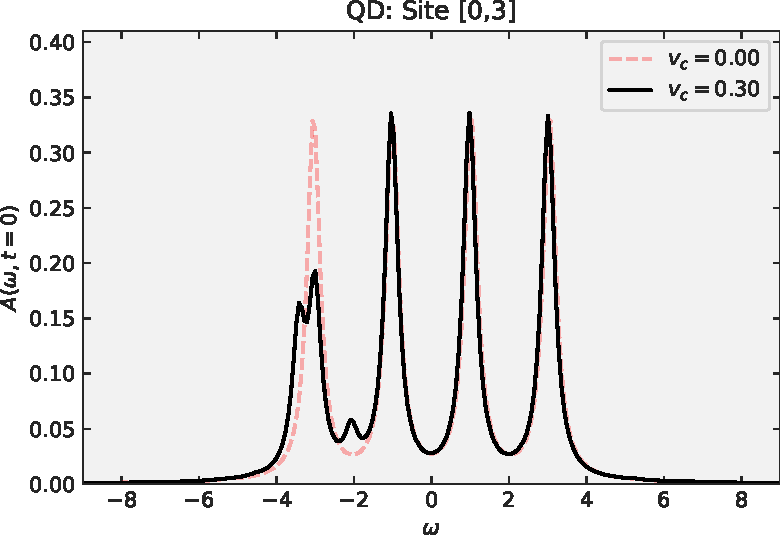
\includegraphics[width=0.49\textwidth]{graph/spectrum_vc_sweep/QD_All_030.pdf}
    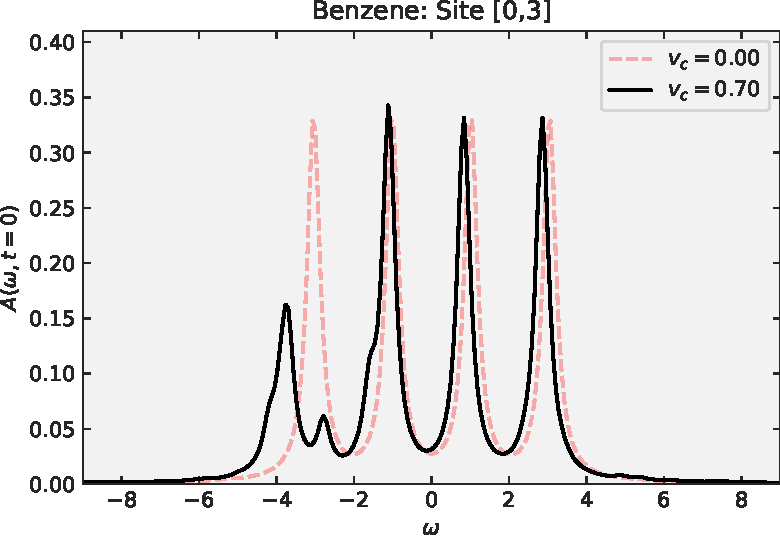
\includegraphics[width=0.49\textwidth]{graph/spectrum_vc_sweep/QD_All_070.pdf}
    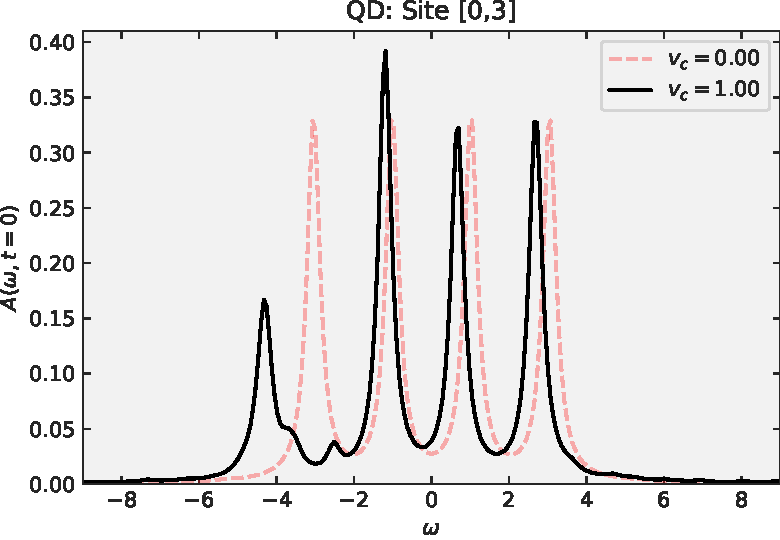
\includegraphics[width=0.49\textwidth]{graph/spectrum_vc_sweep/QD_All_100.pdf}
    \caption{Changes in the spectral function of the QD with increasing coupling $v_c$ to the benzene ring}
    \label{fig:spectrum_vc_sweep_QD}
\end{figure}

\begin{figure}[!hbt]
    \centering
    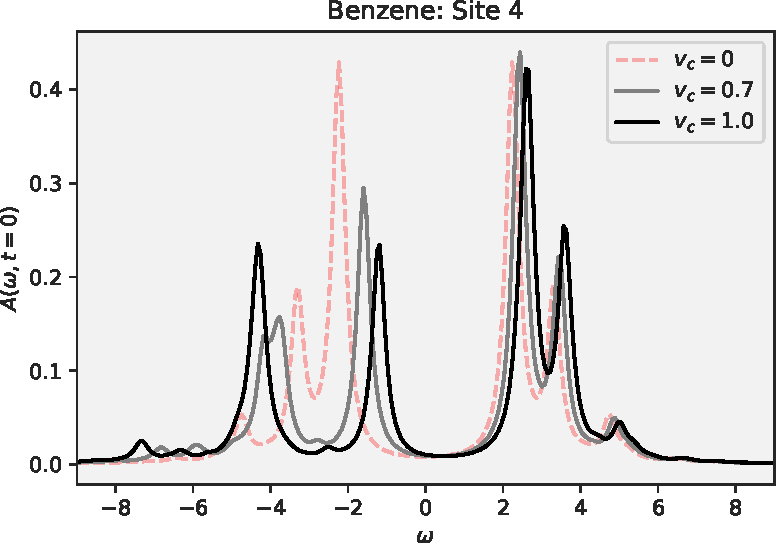
\includegraphics[width=0.43\textwidth]{graph/spectrum_vc_sweep/Benz_4_07_10.pdf}
    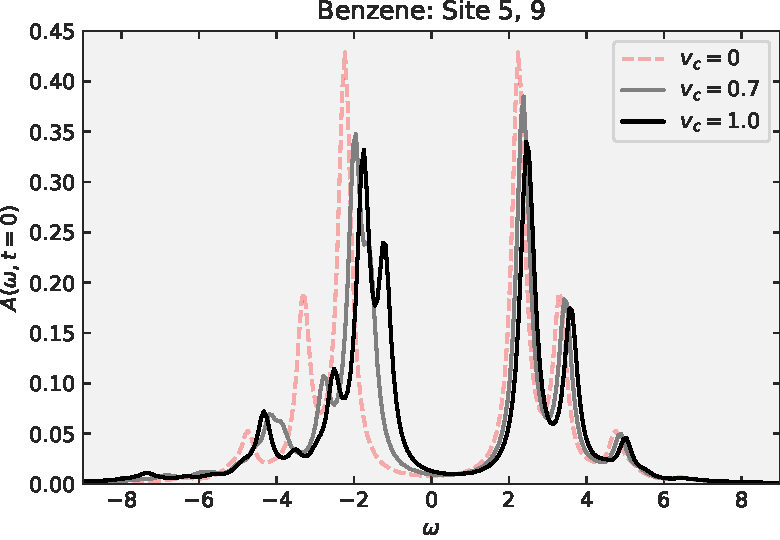
\includegraphics[width=0.43\textwidth]{graph/spectrum_vc_sweep/Benz_59_07_10.pdf}
    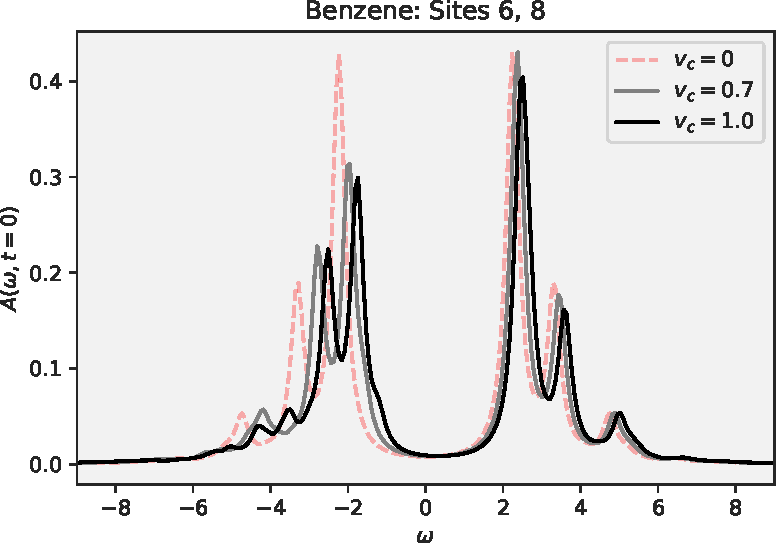
\includegraphics[width=0.43\textwidth]{graph/spectrum_vc_sweep/Benz_68_07_10.pdf}
    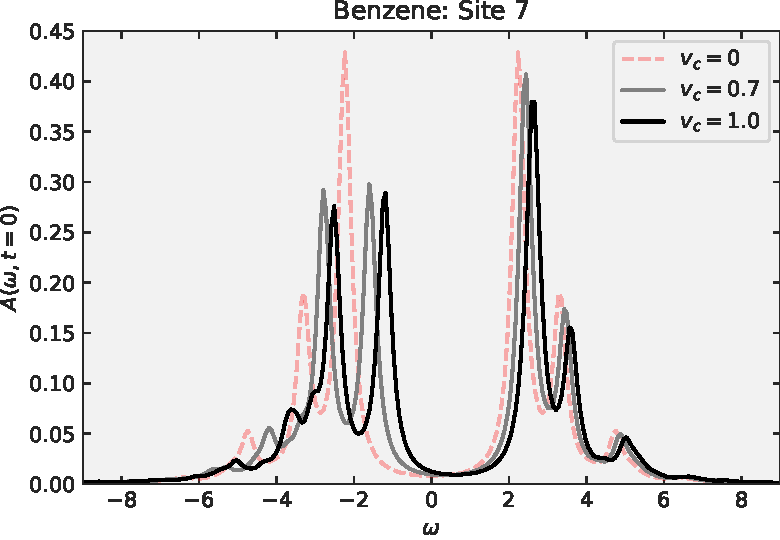
\includegraphics[width=0.43\textwidth]{graph/spectrum_vc_sweep/Benz_7_07_10.pdf}
    \caption{Changes in the spectral function of the benzene ring with increasing coupling $v_c$ to the QD}
    \label{fig:spectrum_vc_sweep_benzene}
\end{figure}

\subsection{Interaction energy and impact ionisation}
Ideally, we would like to investigate the changes in interaction energy on the QD and the benzene ring separately; however, because all the calculations happen in the state basis, and the interaction energy depends on multiple sites, calculating the observable on a particular set of sites is non-trivial. In the state basis, each basis vector is a state of the entire system, and thus all sites are always involved, making it impossible to separate which sites the contributions come from without a change of basis. Performing a transformation into the site basis is outside the scope of this work; thus, we will only be looking at the interaction energy of the system as a whole.
\medskip

Fig. \ref{fig:interaction_energy_omega} shows the interaction energy $\braket{\hat{E}_{\text{int}}}$ for a light pulse with $\omega = 2.00$ and $\omega=4.00$. Once without coupling the QD to benzene ($v_c=0.00$) and once with strong coupling ($v_c=1.00$). The two graphs with $v_c=0.00$ are very similar to the total energy graphs seen in the QD system in Fig. \ref{fig:qd_9_total_energy}. Like before, we see energy transfer at $\omega = 2.00$, but no permanent energy transfer from the light pulse to the system at $\omega = 4.00$, which indicates that no electrons are being promoted to the highest energy level.
\medskip


\begin{figure}[!hbt]
    \centering
    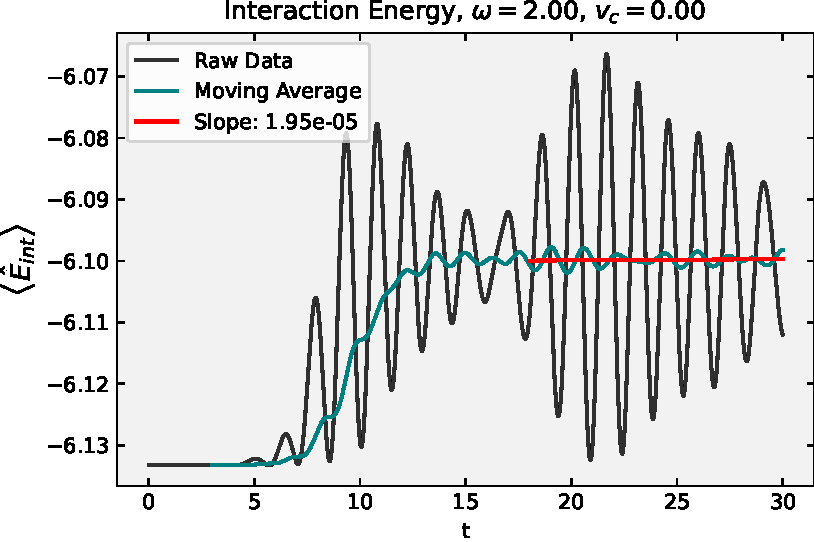
\includegraphics[width=0.44\textwidth]{graph/potential_energy/Epot_w2_vc0.pdf}
    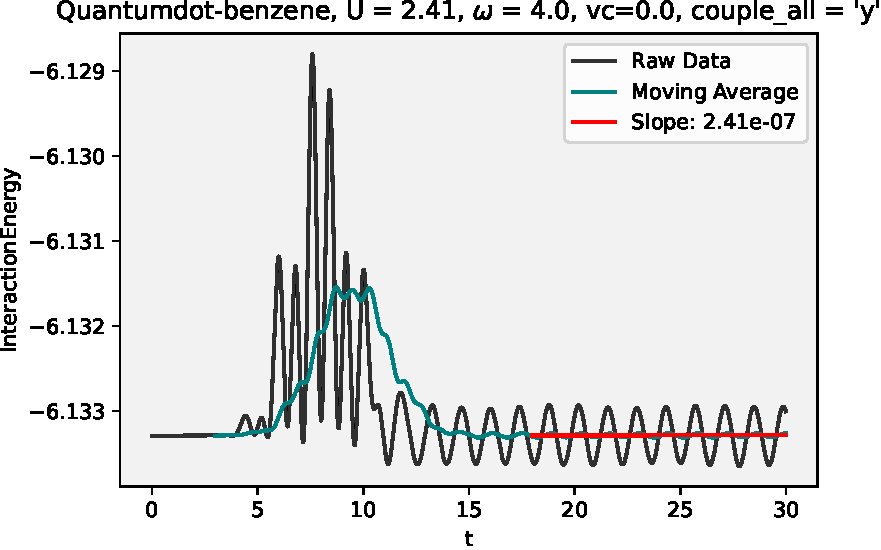
\includegraphics[width=0.44\textwidth]{graph/potential_energy/Epot_w4_vc0.pdf}
    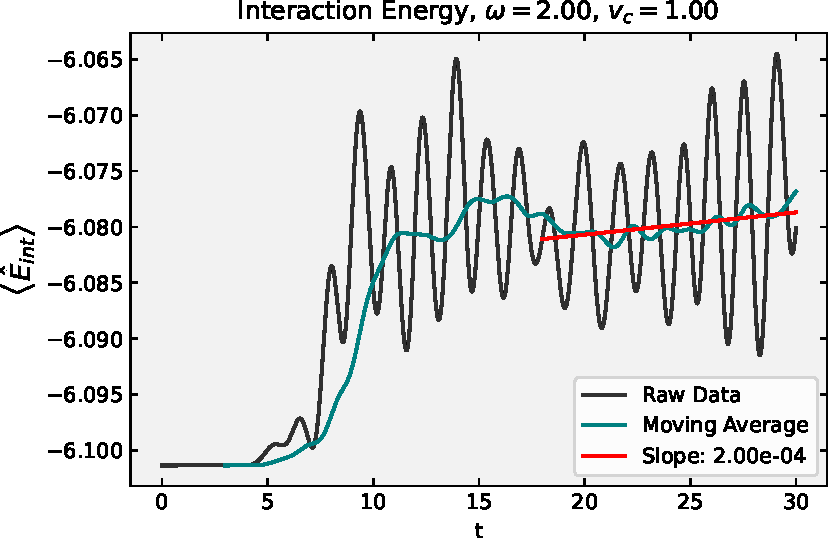
\includegraphics[width=0.44\textwidth]{graph/potential_energy/Epot_w2_vc1.pdf}
    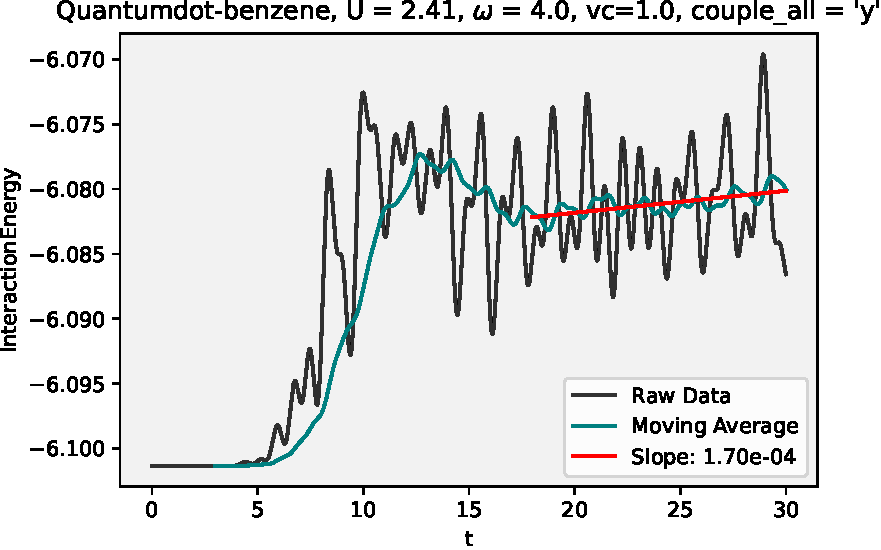
\includegraphics[width=0.44\textwidth]{graph/potential_energy/Epot_w4_vc1.pdf}
    \caption{Interaction energy of coupled system after excitation with light pulse. Shown with strong and without coupling between the QD and benzene.}
    \label{fig:interaction_energy_omega}
\end{figure}
Interestingly when $v_c = 1.0$, we see that for $\omega=4.00$, there is an energy transfer and a steady rise in Interaction energy, even after the pulse has fully decayed, which should generally be an indicator of impact ionisation. Unfortunately, because we can not look at $\braket{\hat{E}_{\text{int}}}$ on a site-wise basis, we can not tell where this effect occurs. However, is look at the occupation numbers per site and attempt to draw conclusions from that.

\subsection{Expected occupation number per site over time}
Even though we can not study the interaction energy on each site individually, it is possible to compute the site-wise occupation numbers $\braket{\hat{n}_i}$ their evolution over time.
\medskip

In Fig. \ref{fig:occupation_vc_00}, we see that for our system, which initially has $1$ electron on each site, the electrons oscillate between sites $0$ and $3$ periodically. For $\omega=4.00$, this oscillation lasts only as long as the pulse duration, but for $\omega=2.00$, it persists since energy was permanently transferred from the pulse to the system. This is consistent with what was observed in Fig. \ref{fig:interaction_energy_omega}.
\medskip

We do not see any changes in occupations numbers on sites $1$ and $2$ due to the symmetry show in Fig. \ref{fig:qd_hoppings}. Because the hopping between sites $0$ and $3$ is set to $v_d = 0$, all electrons moving between the two sites must pass through sites $1$ and $2$. In addition, because the light pulse hits the QD at a $45^\circ$ angle with respect to the lattice, both vertical and horizontal hopping directions experience the same component of the electric field. Due to this, any electrons received from site $1$ are immediately passed onto site $3$ and vice versa, resulting in sites $1$ and $2$ having no occupation number changes. The time evolved occupation numbers for the benzene sites are not shown in Fig. \ref{fig:occupation_vc_00} because they are constant at $\braket{\hat{n}_i} = 1$, because at $v_c = 0$, they do not interact with the light pulse.
\medskip

\begin{figure}[!hbt]
    \centering
    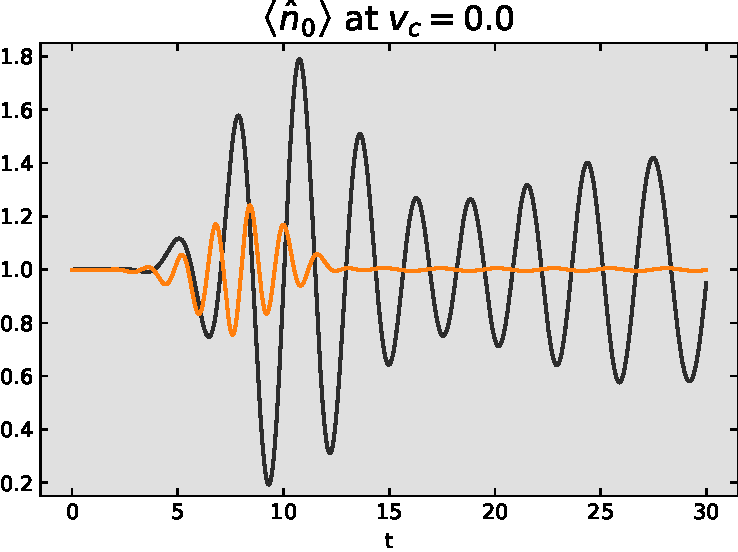
\includegraphics[width=0.43\textwidth]{graph/occupation/occupation_site_0_vc_00.pdf}
    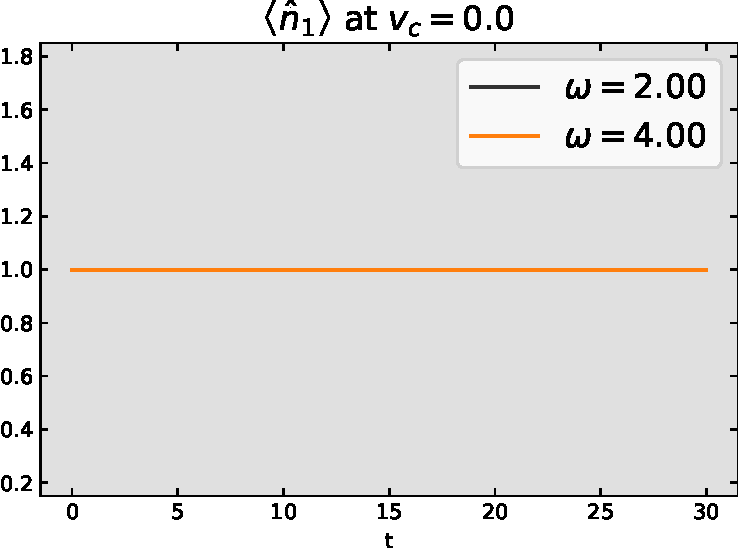
\includegraphics[width=0.43\textwidth]{graph/occupation/occupation_site_1_vc_00.pdf}
    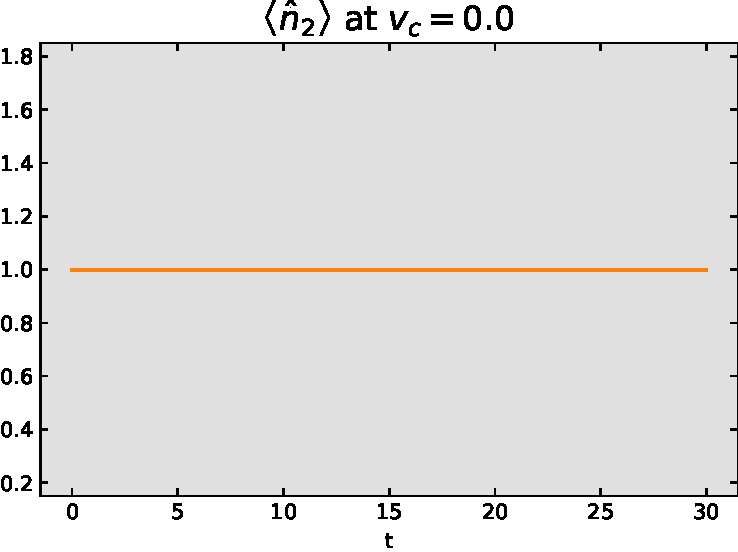
\includegraphics[width=0.43\textwidth]{graph/occupation/occupation_site_2_vc_00.pdf}
    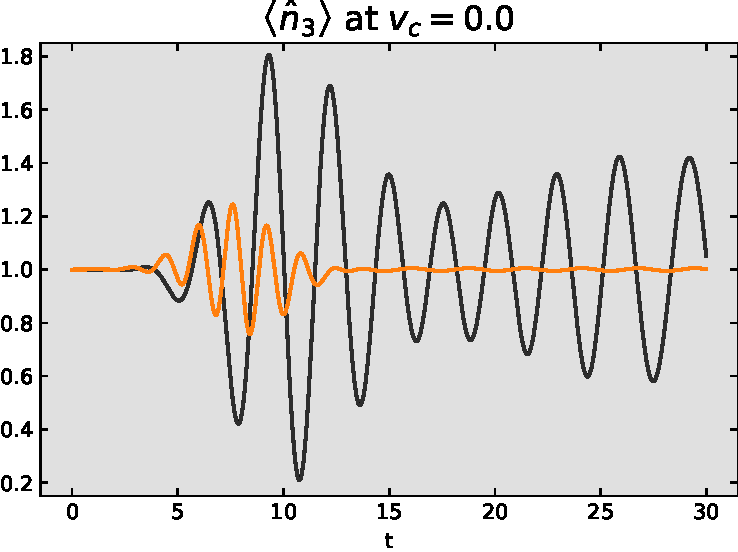
\includegraphics[width=0.43\textwidth]{graph/occupation/occupation_site_3_vc_00.pdf}
    \caption{Occupation numbers of QD sites as a function of time at two different light pulse frequencies. Because $v_c=0.00$ and the benzene ring does not directly interact with the light pulse, all the occupation numbers of the benzene sites remain constant at $1.00$ and thus are not shown in this figure.}
    \label{fig:occupation_vc_00}
\end{figure}

\newpage
When we increase the coupling strength $v_c$, electrons can flow between the QD and the benzene ring. Fig. \ref{fig:occupation_vc_03} and Fig. \ref{fig:occupation_vc_10} show the expected occupation numbers for $v_c=0.30$ and $v_c=1.00$ respectively. The figures are laid out to reflect the geometry of the coupled system, like the diagram in Fig. \ref{fig:coupled_distances} turned $90^\circ$ clockwise. Note that the $y$-axis scaling is different on the QD sites compared to the benzene sites since the occupation changes are smaller on benzene.
\medskip

\begin{figure}[!hbt]
 \makebox[\textwidth]{\makebox[1.20\textwidth]{ % to overflow the margins
    \begin{minipage}[b]{.59\textwidth}
                \centering
                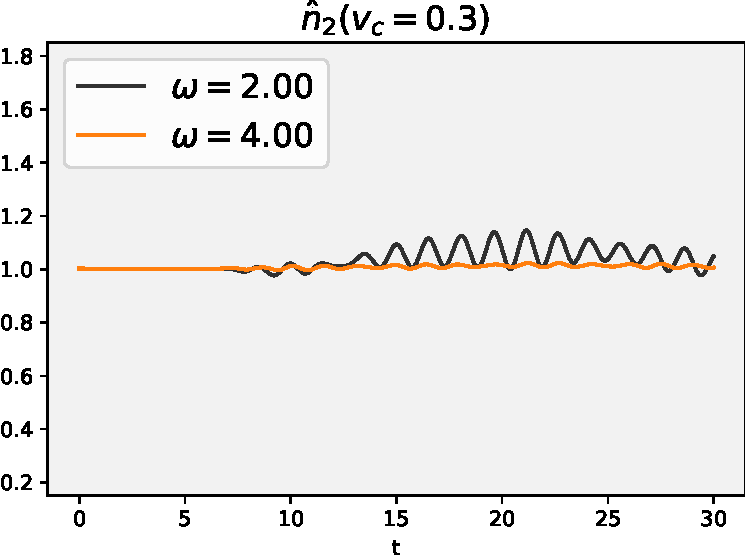
\includegraphics[trim=0 0 0 -4, clip, width=0.49\textwidth]{graph/occupation/occupation_site_2_vc_03.pdf}
                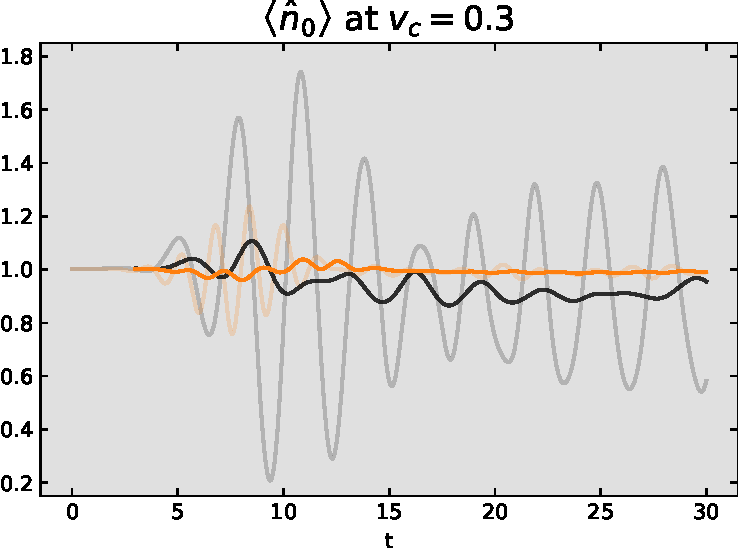
\includegraphics[trim=0 0 0 -4, clip, width=0.49\textwidth]{graph/occupation/occupation_site_0_vc_03.pdf}
                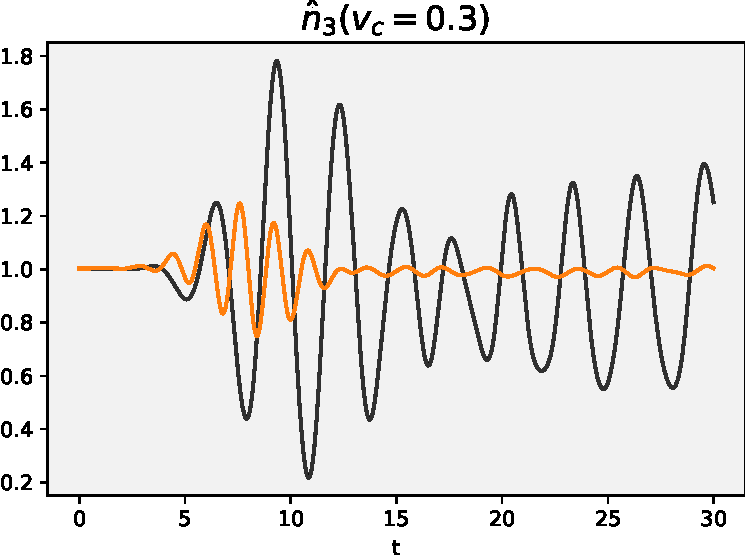
\includegraphics[trim=0 0 0 -4, clip, width=0.49\textwidth]{graph/occupation/occupation_site_3_vc_03.pdf}
                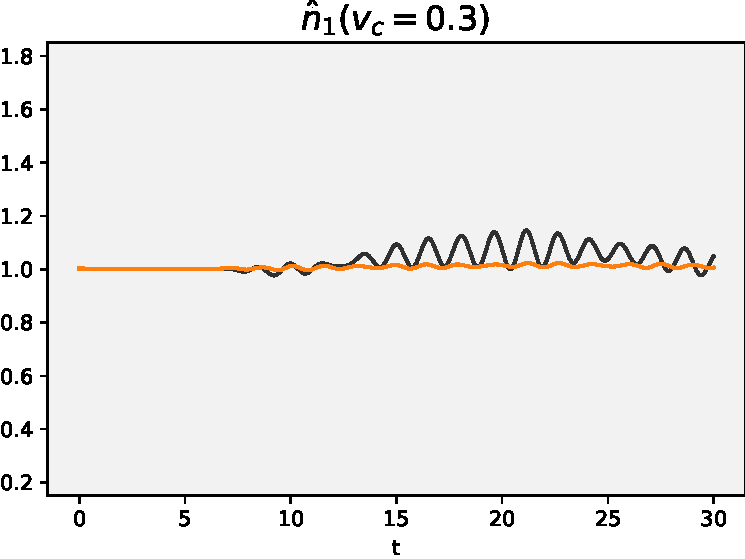
\includegraphics[trim=0 0 0 -4, clip, width=0.49\textwidth]{graph/occupation/occupation_site_1_vc_03.pdf}
                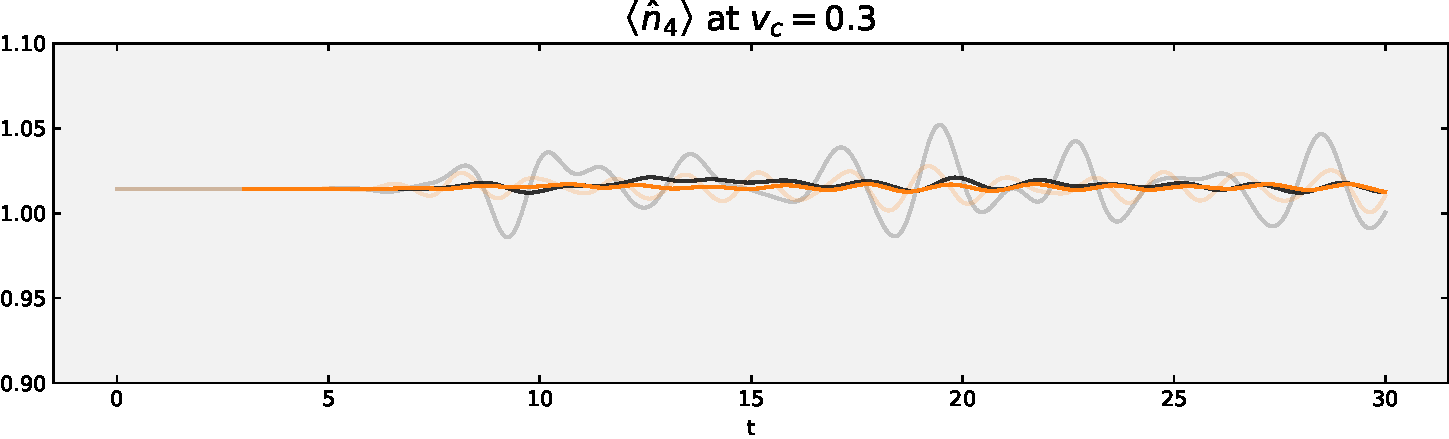
\includegraphics[trim=0 0 0 -4, clip, width=1.00\textwidth]{graph/occupation/occupation_site_4_vc_03.pdf}
                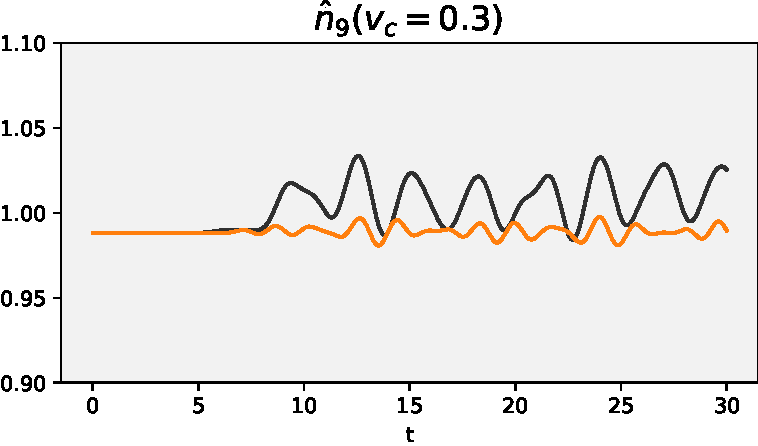
\includegraphics[trim=0 0 0 -4, clip, width=0.49\textwidth]{graph/occupation/occupation_site_9_vc_03.pdf}
                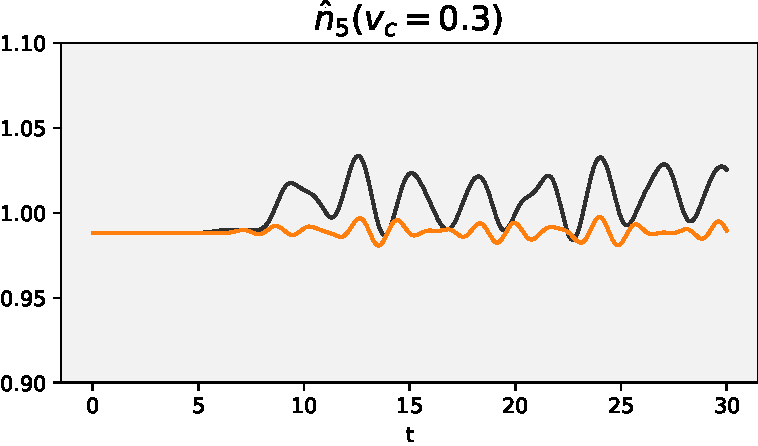
\includegraphics[trim=0 0 0 -4, clip, width=0.49\textwidth]{graph/occupation/occupation_site_5_vc_03.pdf}
                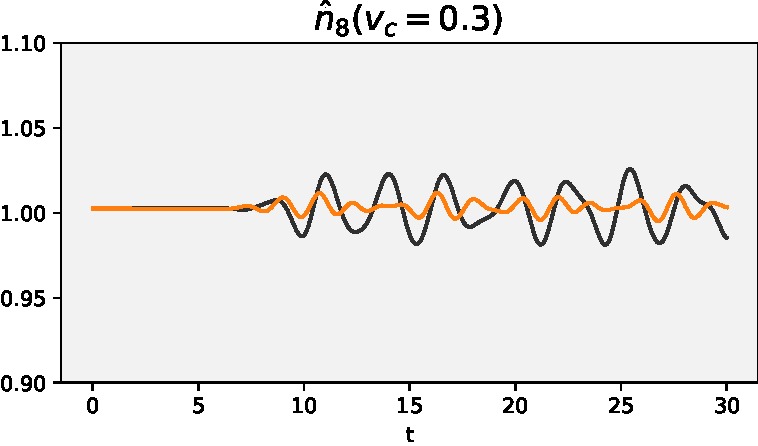
\includegraphics[trim=0 0 0 -4, clip, width=0.49\textwidth]{graph/occupation/occupation_site_8_vc_03.pdf}
                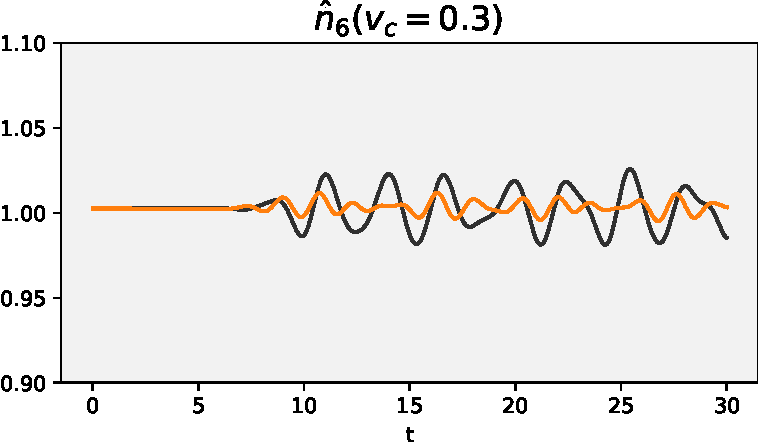
\includegraphics[trim=0 0 0 -4, clip, width=0.49\textwidth]{graph/occupation/occupation_site_6_vc_03.pdf}
                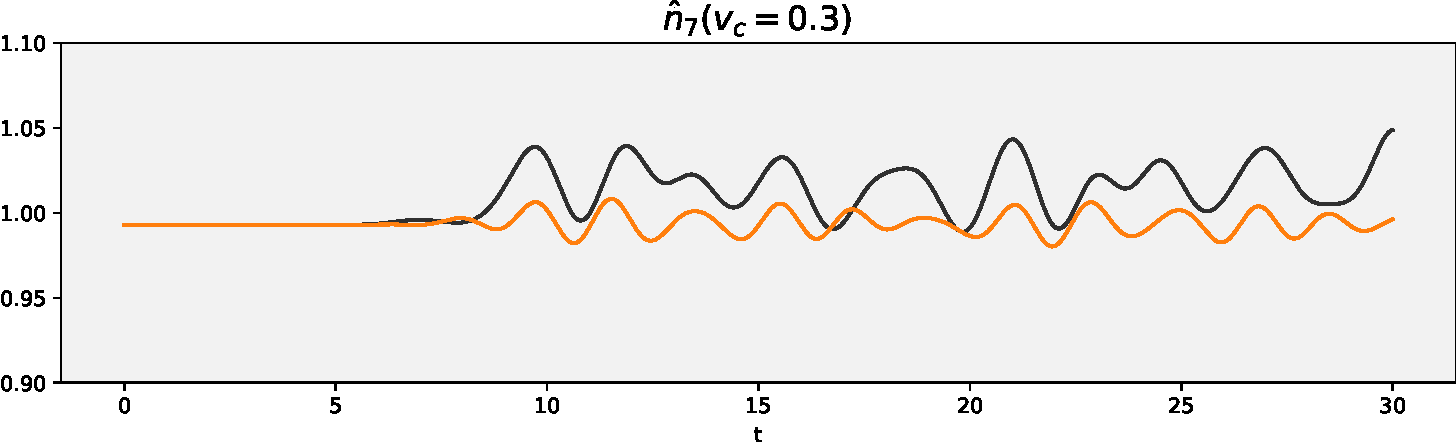
\includegraphics[trim=0 0 0 -4, clip, width=1.00\textwidth]{graph/occupation/occupation_site_7_vc_03.pdf}
       \caption{Expectation of occupation numbers for the coupled system at $v_c = 0.3$. Darker lines are moving averages of the raw data shown in a lower opacity.}
        \label{fig:occupation_vc_03}
    \end{minipage}
    \hfill
    \begin{minipage}[b]{.59\textwidth}
                \centering
                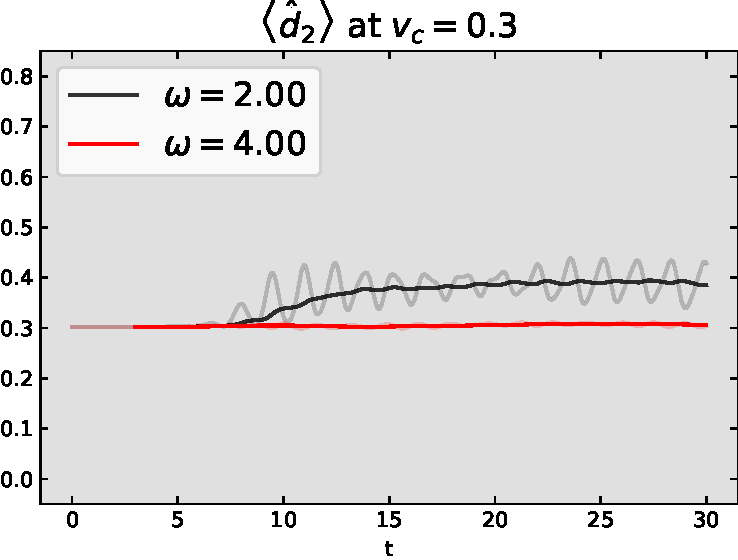
\includegraphics[width=0.49\textwidth]{graph/double_occupation/double_occupation_vc_03_site_2.pdf}
                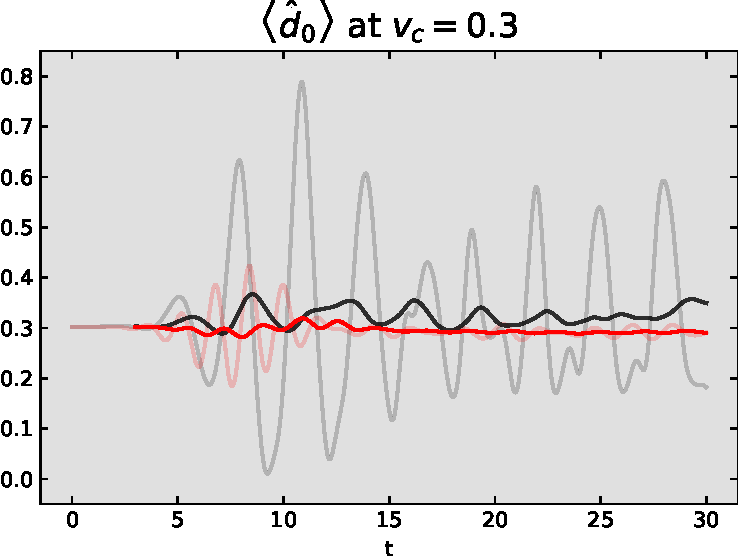
\includegraphics[width=0.49\textwidth]{graph/double_occupation/double_occupation_vc_03_site_0.pdf}
                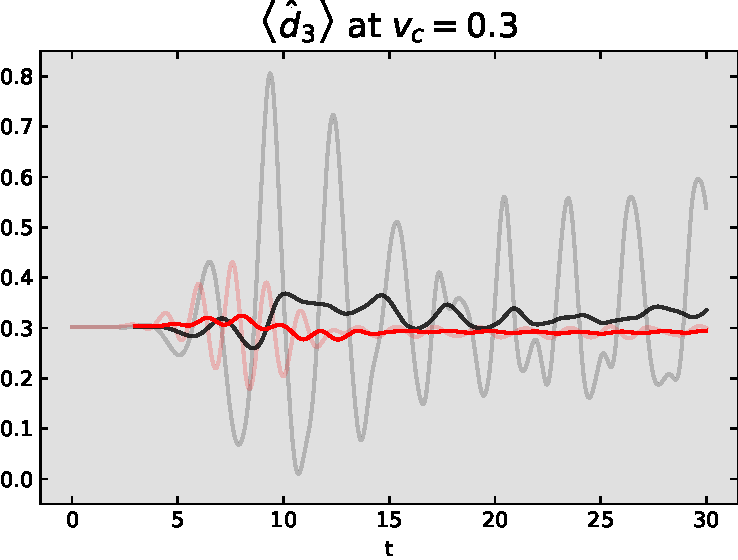
\includegraphics[width=0.49\textwidth]{graph/double_occupation/double_occupation_vc_03_site_3.pdf}
                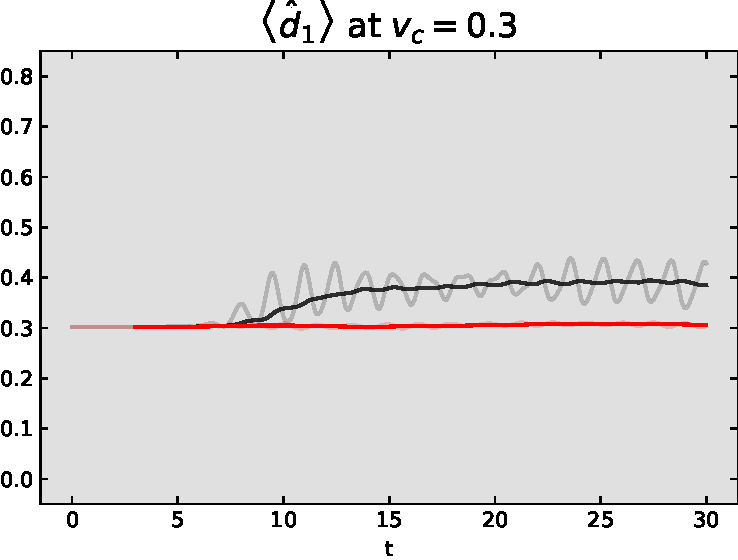
\includegraphics[width=0.49\textwidth]{graph/double_occupation/double_occupation_vc_03_site_1.pdf}
                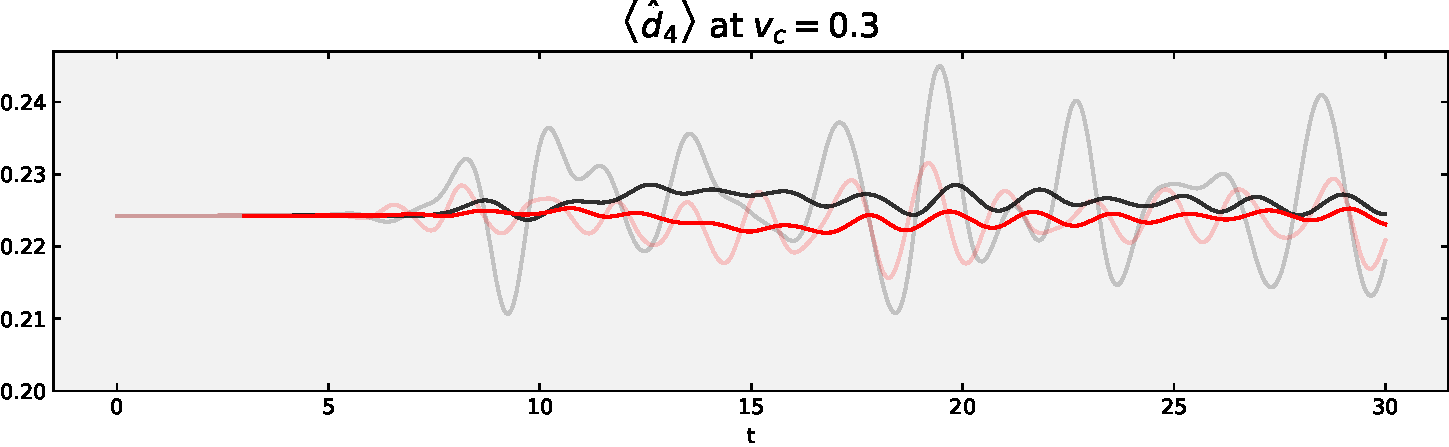
\includegraphics[width=1.00\textwidth]{graph/double_occupation/double_occupation_vc_03_site_4.pdf}
                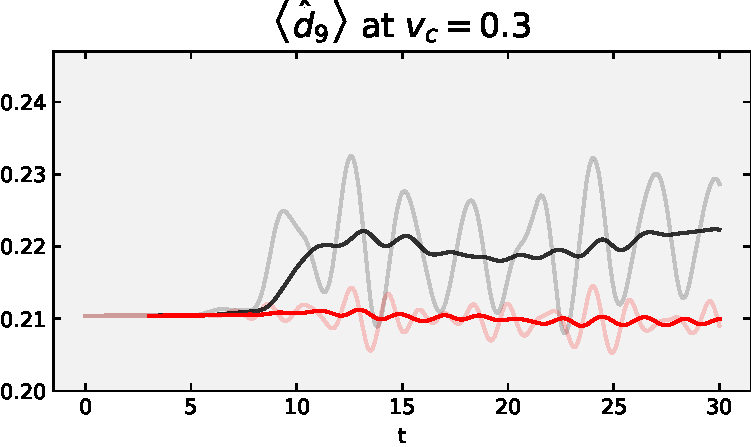
\includegraphics[width=0.49\textwidth]{graph/double_occupation/double_occupation_vc_03_site_9.pdf}
                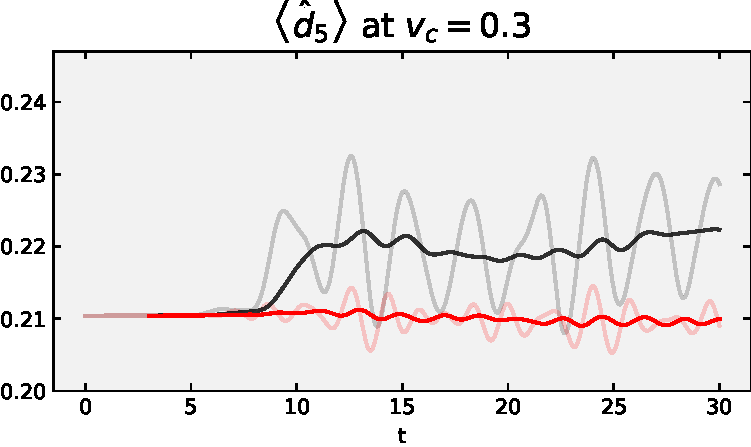
\includegraphics[width=0.49\textwidth]{graph/double_occupation/double_occupation_vc_03_site_5.pdf}
                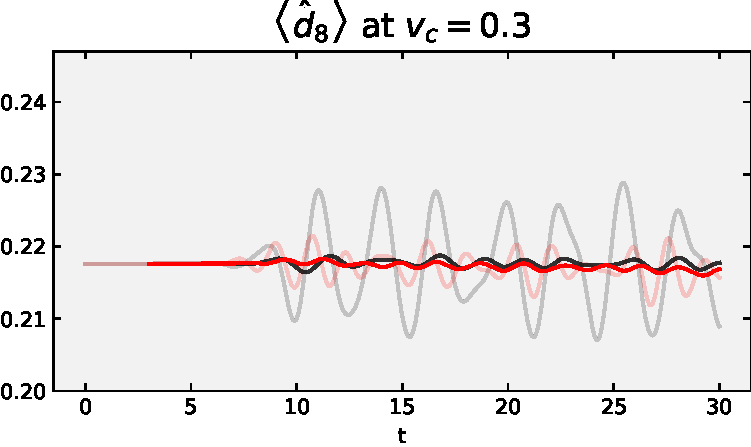
\includegraphics[width=0.49\textwidth]{graph/double_occupation/double_occupation_vc_03_site_8.pdf}
                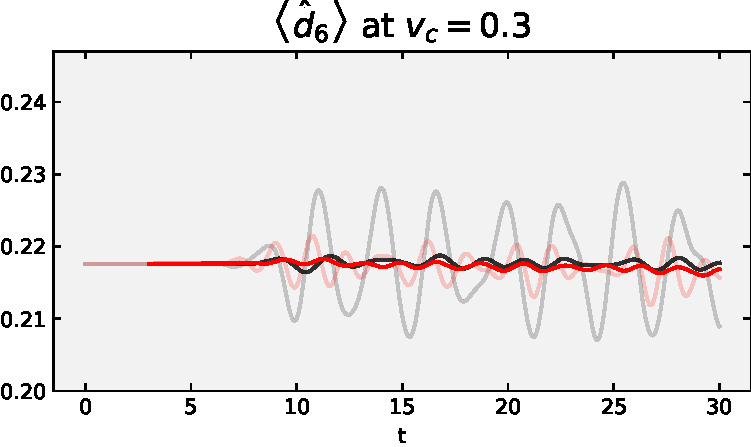
\includegraphics[width=0.49\textwidth]{graph/double_occupation/double_occupation_vc_03_site_6.pdf}
                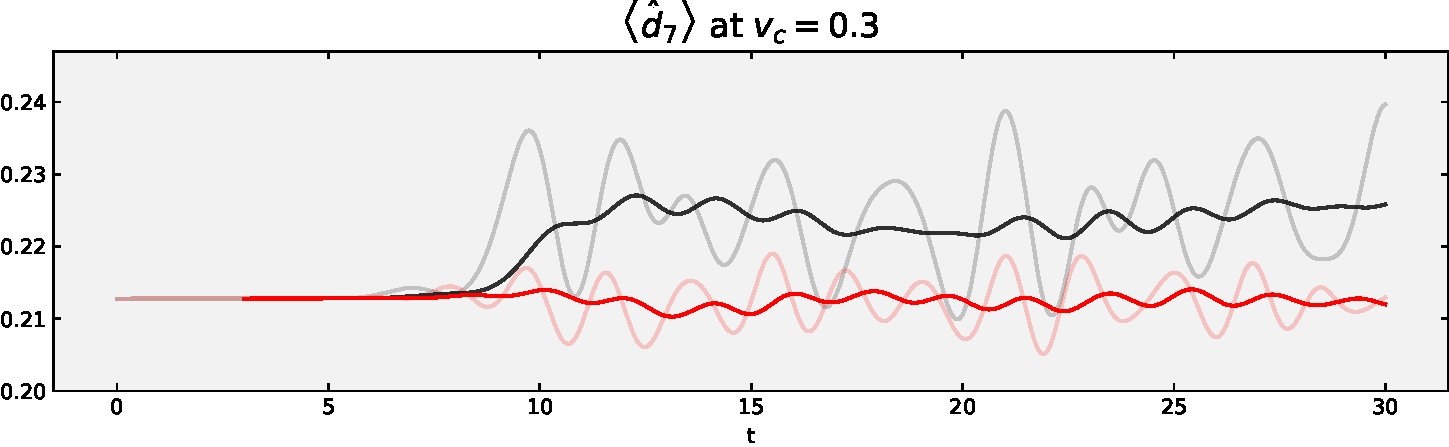
\includegraphics[width=1.00\textwidth]{graph/double_occupation/double_occupation_vc_03_site_7.pdf}
        \caption{Expectation of double occupation numbers for the coupled system at $v_c = 0.3$.\newline}
        \label{fig:double_occupation_vc_03}
    \end{minipage}}}
\end{figure}
\newpage

\begin{figure}[!hbt]
 \makebox[\textwidth]{\makebox[1.20\textwidth]{ % to overflow the margins
    \begin{minipage}[b]{.59\textwidth}
                \centering
                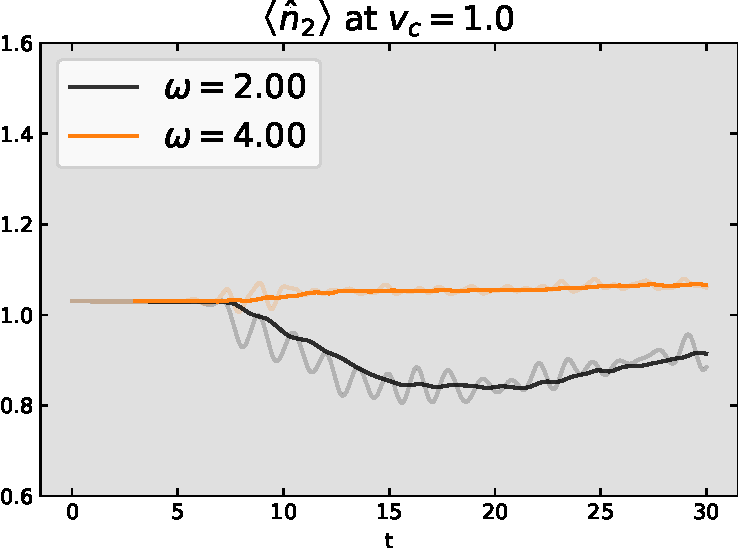
\includegraphics[trim=0 0 0 -4, clip, width=0.49\textwidth]{graph/occupation/occupation_site_2_vc_10.pdf}
                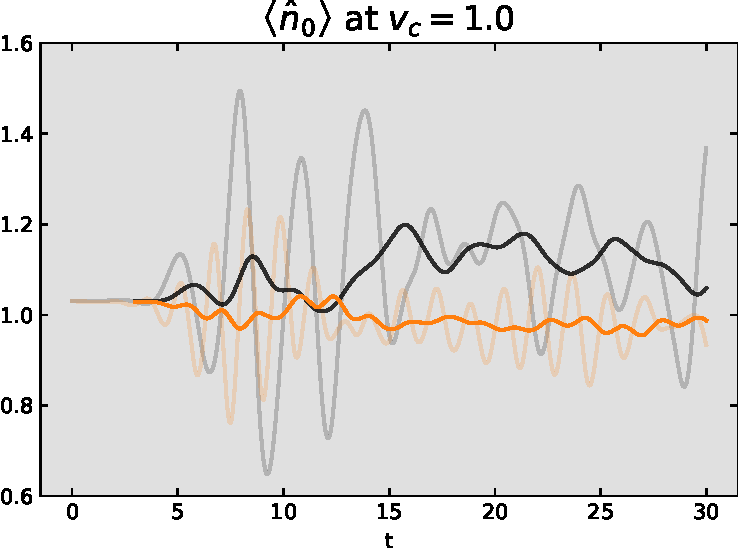
\includegraphics[trim=0 0 0 -4, clip, width=0.49\textwidth]{graph/occupation/occupation_site_0_vc_10.pdf}
                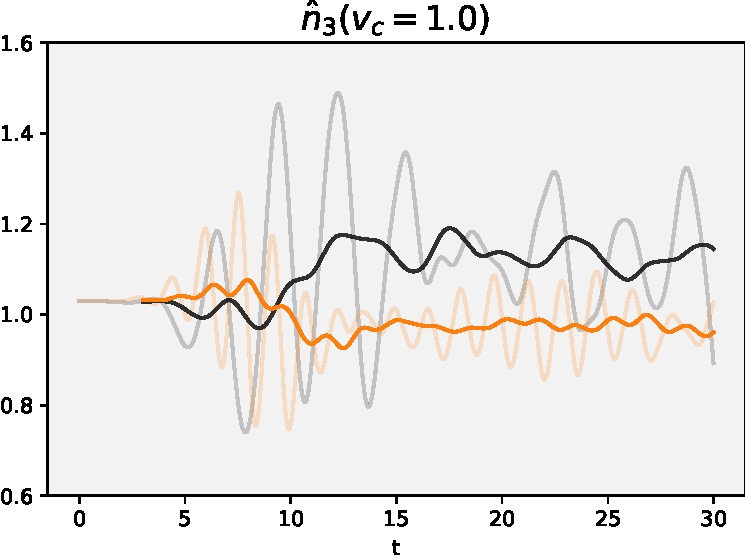
\includegraphics[trim=0 0 0 -4, clip, width=0.49\textwidth]{graph/occupation/occupation_site_3_vc_10.pdf}
                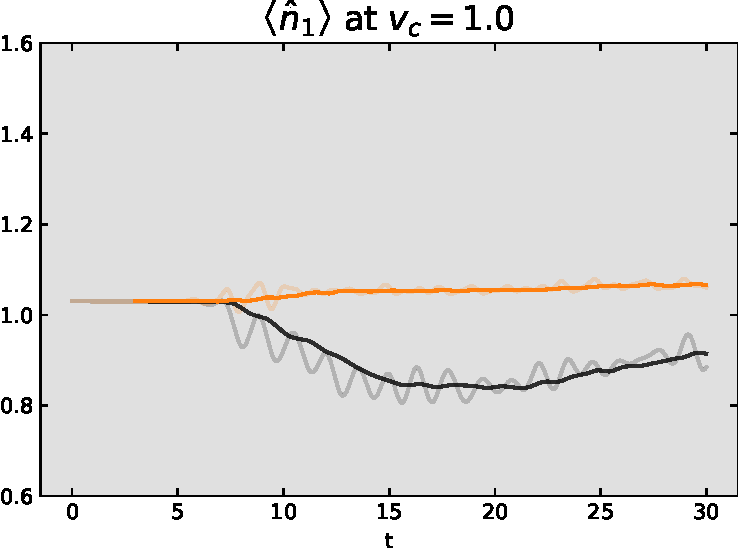
\includegraphics[trim=0 0 0 -4, clip, width=0.49\textwidth]{graph/occupation/occupation_site_1_vc_10.pdf}
                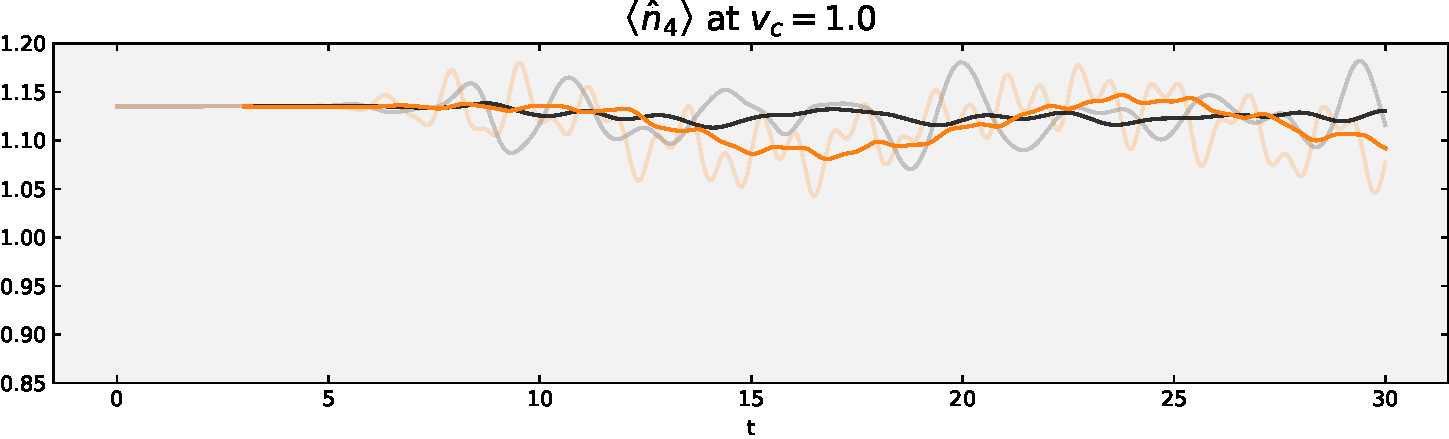
\includegraphics[trim=0 0 0 -4, clip, width=1.00\textwidth]{graph/occupation/occupation_site_4_vc_10.pdf}
                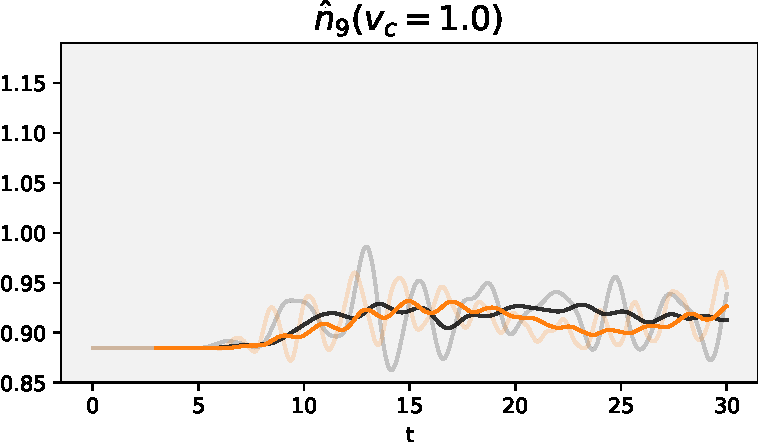
\includegraphics[trim=0 0 0 -4, clip, width=0.49\textwidth]{graph/occupation/occupation_site_9_vc_10.pdf}
                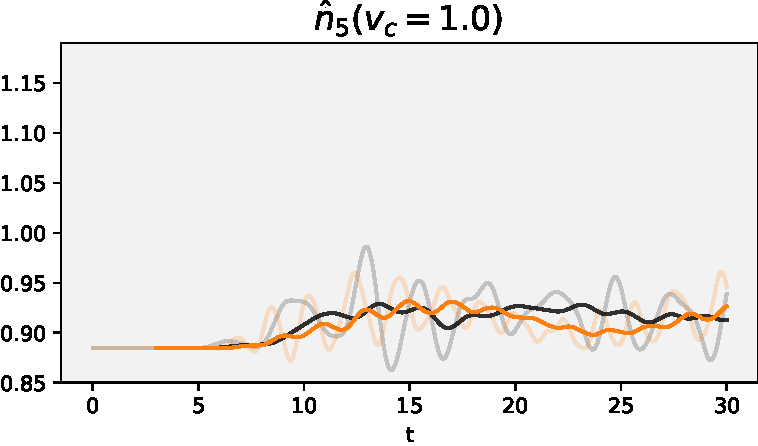
\includegraphics[trim=0 0 0 -4, clip, width=0.49\textwidth]{graph/occupation/occupation_site_5_vc_10.pdf}
                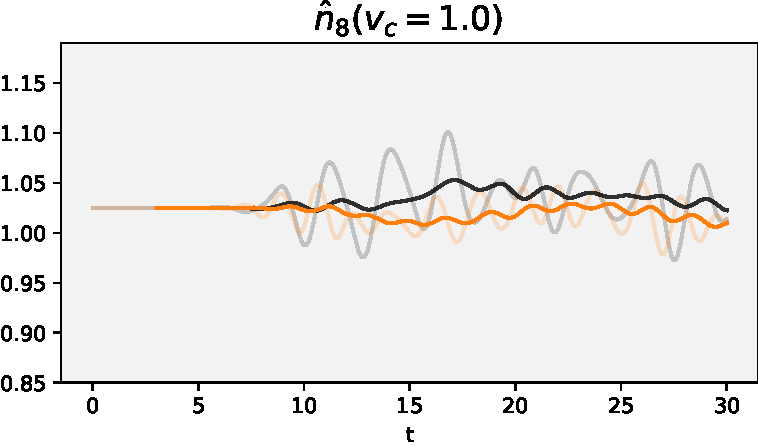
\includegraphics[trim=0 0 0 -4, clip, width=0.49\textwidth]{graph/occupation/occupation_site_8_vc_10.pdf}
                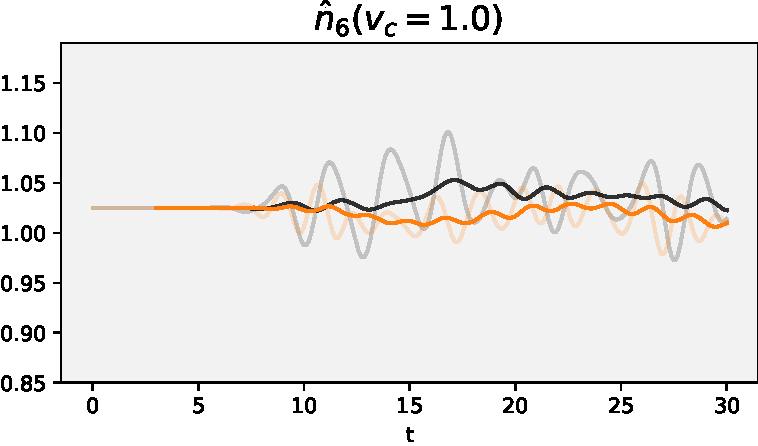
\includegraphics[trim=0 0 0 -4, clip, width=0.49\textwidth]{graph/occupation/occupation_site_6_vc_10.pdf}
                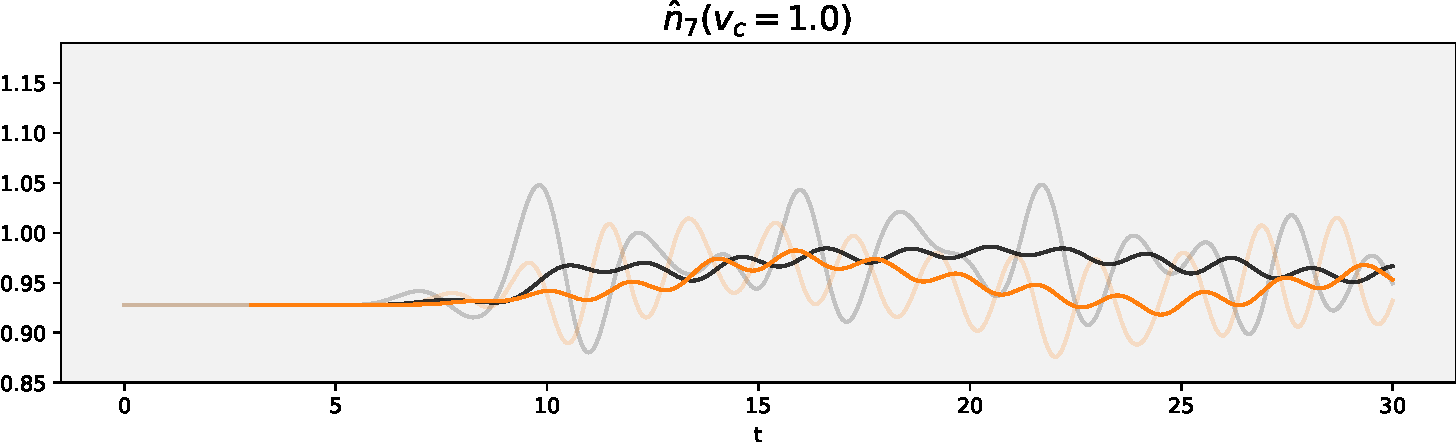
\includegraphics[trim=0 0 0 -4, clip, width=1.00\textwidth]{graph/occupation/occupation_site_7_vc_10.pdf}
       \caption{Expectation of occupation numbers for the coupled system at $v_c = 1.0$. Darker lines are moving averages of the raw data shown in a lower opacity.}
        \label{fig:occupation_vc_10}
    \end{minipage}
    \hfill
    \begin{minipage}[b]{.59\textwidth}
                \centering
                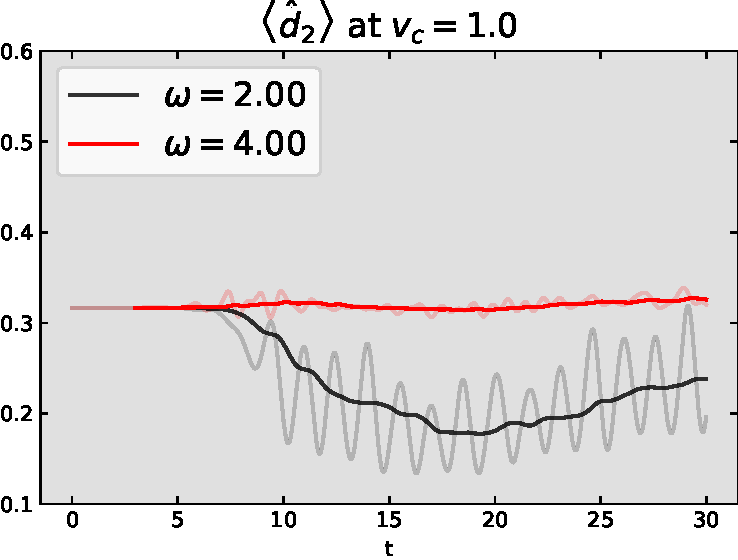
\includegraphics[width=0.49\textwidth]{graph/double_occupation/double_occupation_vc_10_site_2.pdf}
                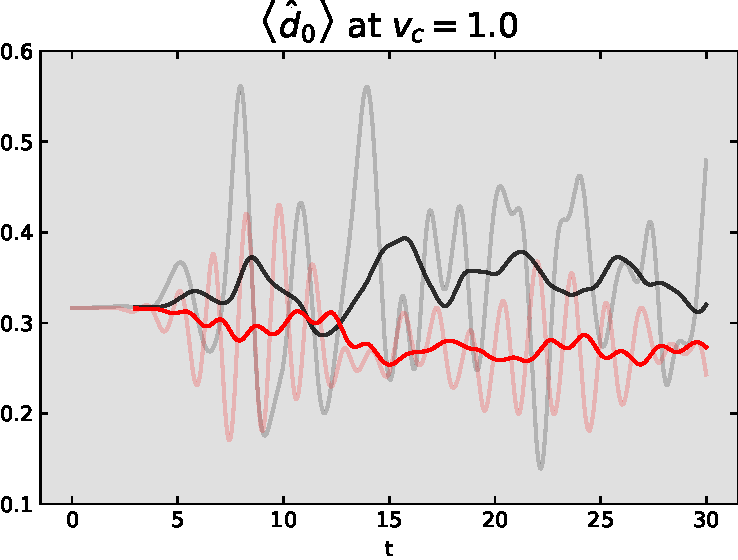
\includegraphics[width=0.49\textwidth]{graph/double_occupation/double_occupation_vc_10_site_0.pdf}
                \includegraphics[width=0.49\textwidth]{graph/double_occupation/double_occupation_vc_10_site_3.pdf}
                \includegraphics[width=0.49\textwidth]{graph/double_occupation/double_occupation_vc_10_site_1.pdf}
                \includegraphics[width=1.00\textwidth]{graph/double_occupation/double_occupation_vc_10_site_4.pdf}
                \includegraphics[width=0.49\textwidth]{graph/double_occupation/double_occupation_vc_10_site_9.pdf}
                \includegraphics[width=0.49\textwidth]{graph/double_occupation/double_occupation_vc_10_site_5.pdf}
                \includegraphics[width=0.49\textwidth]{graph/double_occupation/double_occupation_vc_10_site_8.pdf}
                \includegraphics[width=0.49\textwidth]{graph/double_occupation/double_occupation_vc_10_site_6.pdf}
                \includegraphics[width=1.00\textwidth]{graph/double_occupation/double_occupation_vc_10_site_7.pdf}
       \caption{Expectation of double occupation numbers for the coupled system at $v_c = 1.0$.\newline}
        \label{fig:double_occupatino_vc_10}
    \end{minipage}}}
\end{figure}
\newpage

Fig. \ref{fig:occupation_vc_03}, in particular, reveals significant occupation increases on the benzene ring sites $7, 5$ and $9$ at $\omega=2.00$.  Moreover, in Fig. \ref{fig:double_occupation_vc_03}, we see that from $t=20$ onward, there is a steady rise in double occupation on those sites as well. Even though section \ref{sec:interaction_energy} pointed out why double occupation is no longer a good measure for impact ionisation, seeing this steady increase after the pulse has decayed is still a weaker indication that impact ionisation may be taking place on the benzene ring.

\subsection{Electron transfer between QD and benzene} \label{subsec:electron_transfer_QD_benzene}
In order to get a clearer picture of the electron currents between the QD and benzene subsystems than the site-wise occupation numbers from the previous section can provide, we calculate the sums of occupation number expectation values on all QD and all benzene sites. This allows us to study the net electron transfer between the two coupled systems.
\medskip

All changes in the expected occupation numbers are calculated with respect to their occupation numbers at half-filling. This means that for the QD, $4$ electrons were subtracted off the occupation number, and $6$ electrons were subtracted from the occupation number of the benzene ring.
%
\begin{equation}
    \begin{split}
        \braket{\Delta\hat{n}_{\text{QD}}}(t) = \left(\sum_{i=0}^3 \braket{\hat{n}_i}(t) \right) - 4\\
        \braket{\Delta\hat{n}_{\text{benz}}}(t) = \left(\sum_{i=4}^9 \braket{\hat{n}_i}(t) \right) - 6
    \end{split}
\end{equation}
%
Fig. \ref{fig:occupation_sum_w_2_vc_03} shows that, as expected, the total number of electrons is conserved and that for $v_c=0.30$ and $\omega=2.00$, there is a clear flow of electrons from the QD to the benzene ring, even after the pulse has fully decayed. This flow of electrons from the QD to benzene from roughly $t=16$ onward coincides with the possible impact ionisation seen in the previous section. Because simply having more electrons on the benzene ring will lead to more double occupations, we can not clearly say which parts of the double occupancy increases are due to impact ionisation and which are due to the electron currents.

\begin{figure}[!hbt]
    \centering
    \includegraphics[width=0.6\textwidth]{graph/occupation/occupation_w2_03_sum.pdf}
    \caption{Changes in expected occupation number between QD an Benzene over time.}
    \label{fig:occupation_sum_w_2_vc_03}
\end{figure}


Fig. \ref{fig:occupation_qd_benzene_sum_vcsweep} shows the occupation number changes on benzene for various coupling strengths. In addition to again seeing an increases in occupation after the pulse, there is also clear dependence of the occupation numbers at $t=0$ on the coupling strength. This makes sense because at $t=0$ the system is in its ground state and for this calculation the on-site Coulomb interaction term $U_{ii}$ was chosen differently on QD sites and on Benzene sites. With $U_{ii}^{\text{QD}} = 2.406$ and $U_{ii}^{\text{Benz}} = 3.962$, the energy cost of moving electrons form benzene to the QD is outweighed by the energy savings of having less electrons undergoing Coulomb interactions on the benzene ring, thus in the ground state $\Delta \braket{\hat{n}_{\text{Benz}}} < 0$ for $v_c > 0$.

\begin{figure}[!hbt]
    \centering
    \includegraphics[width=0.49\textwidth]{graph/occupation/occupation_w2_Benz_sum_vcsweep.pdf}
    \includegraphics[width=0.49\textwidth]{graph/occupation/occupation_w4_Benz_sum_vcsweep.pdf}
    \caption{Changes in expected occupation numbers for the benzene-subsystem at pulse frequencies $\omega=2, 4$ for various coupling strengths $v_c$.}
    \label{fig:occupation_qd_benzene_sum_vcsweep} 
\end{figure}

This also explains the shifting of the QD and benzene spectra with changing $v_c$ in Figs. \ref{fig:spectrum_vc_sweep_QD} and \ref{fig:spectrum_vc_sweep_benzene}. The reduction in benzene's occupation numbers in the ground state can be seen as due to the up-shift in its energy levels, and because the energy levels in the QD are shifted downwards the ground state occupation increases.


\section{Conclusion}
In this work, we attempted to simulate an experimentally realisable system of a quantum dot coupled to a benzene ring and investigate its behaviour under photoexcitation by a light pulse, particularly in search of impact ionisation. However, the desired effects could not be clearly demonstrated. The final result is complicated because impact ionisation could not be clearly identified in any single part of the system; instead, we see a mixture of effects on both the quantum dot and the benzene ring. Partially due to impact ionisation and partially due to charge transfer, which for now seem inseparably connected with each other. Further developments in the methodology for analysing this system will be needed to better understand the true mechanisms at work.